% TOMLSignals — IEEE MLSP 2026
% Transistor-Level Energy Analysis of Signal Processing Algorithms
\documentclass{article}
\usepackage{amsmath,graphicx,mlspconf}
\usepackage{xcolor}
\usepackage{booktabs}
\usepackage{url}
\usepackage{multirow}

% Copyright notice (use notice 4 for non-government authors)
\copyrightnotice{979-8-3503-2411-2/25/\$31.00 {\copyright}2025 IEEE}

% Header
\toappear{2026 IEEE International Workshop on Machine Learning for Signal Processing, Sep.\ 28-- Oct.\ 1, 2026, Atlanta, USA}

% Double-blind submission
\name{Anonymous}
\address{Anonymous}

% Camera-ready (uncomment when accepted):
%\name{Muntaser Syed$^{\star\dagger}$%
%  \qquad Marius Silaghi$^{\star}$%
%  \qquad Sheikh Abujar$^{\dagger}$%
%  \qquad Sharun Akter Khushbu$^{\ddagger}$}
%\address{%
%  $^{\star}$ Florida Institute of Technology, Melbourne, FL, USA\\%
%  $^{\dagger}$ University of Alabama at Birmingham, Birmingham, AL, USA\\%
%  $^{\ddagger}$ Daffodil International University, Dhaka, Bangladesh}

\title{Transistor-Level Energy Analysis of Signal Processing Algorithms: Beyond Operation Counting}

\begin{document}
\ninept
\maketitle

\begin{abstract}
Accurate energy prediction for signal processing algorithms is critical for resource-constrained and energy-aware systems, yet existing approaches rely on floating-point operation counts that ignore memory hierarchy costs, sequential dispatch overhead, and hardware implementation details. We present a physics-grounded energy model based on Transistor Operations (TOs), validated across 37 signal processing algorithms spanning 8 categories on two NVIDIA GPUs (RTX 4090 Laptop and A100 SXM4). Our four-parameter model achieves $r^2 = 0.947$ (RTX 4090) and $r^2 = 0.982$ (A100) with 80\% head-to-head ranking accuracy. Nsight Compute hardware profiling validates key corrections including split-radix FFT operation counts (99.4\% match) and complex MAC reduction on FMA hardware (99.2\% match). We identify three distinct energy regimes for sequential algorithms --- parallel, Python-loop dispatch, and fused-sequential --- with a 1{,}190$\times$ energy gap between dispatch modes. A systematic CPU-vs-GPU comparison across all 37 algorithms reveals that sequential algorithms are 10--100$\times$ more energy-efficient on CPU, challenging the assumption that GPUs are universally superior for compute.
\end{abstract}

\begin{keywords}
Energy efficiency, signal processing, GPU, transistor operations, power measurement
\end{keywords}

% =========================================================================
\section{Introduction}
\label{sec:intro}
% =========================================================================

% TODO: Write introduction
% - Energy problem in signal processing
% - Limitations of FLOP counting
% - Contributions of this paper

% =========================================================================
\section{TOML Framework}
\label{sec:framework}
% =========================================================================

% TODO: TO cost table (consistent with FLAIRS, TOMLCloud)
% 4-parameter model derivation with physical justification

% =========================================================================
\section{Experimental Setup}
\label{sec:setup}
% =========================================================================

% TODO: 37 algorithms across 8 categories
% Two GPUs, thermal settling protocol
% Nsight Compute validation methodology
% CPU measurement via RAPL

% =========================================================================
\section{Results}
\label{sec:results}
% =========================================================================

% TODO: r² = 0.947/0.982
% 80% ranking accuracy
% Cross-GPU α consistency
% NCU validation
% Three sequential energy regimes

% --- Fig 1: Predicted vs Measured ---
%\begin{figure}[t]
%\centering
%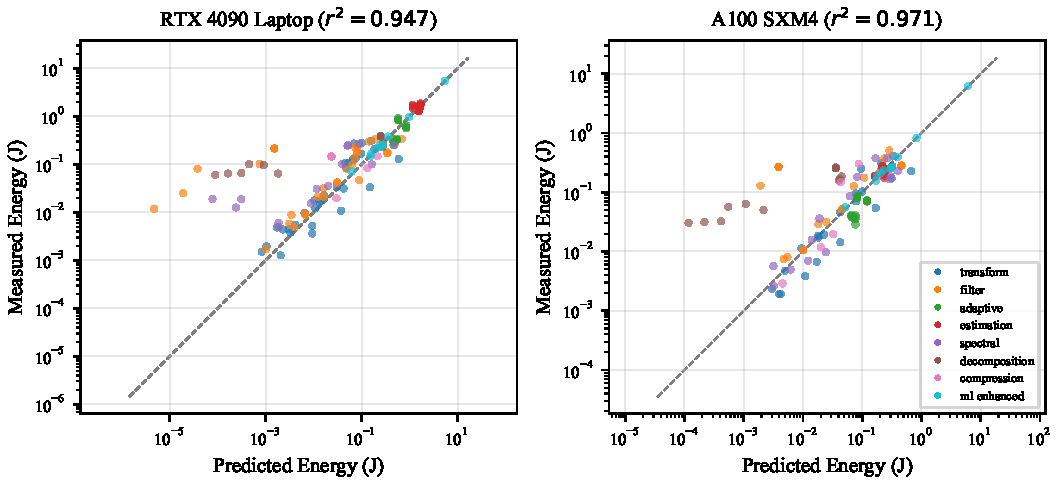
\includegraphics[width=\columnwidth]{figures/fig1_scatter}
%\caption{TOML predicted vs.\ measured energy (log-log) for 37 signal processing algorithms on two GPUs. The four-parameter model achieves $r^2 = 0.947$ (RTX 4090) and $r^2 = 0.982$ (A100).}
%\label{fig:scatter}
%\end{figure}

% =========================================================================
\section{CPU vs GPU Analysis}
\label{sec:cpugpu}
% =========================================================================

% TODO: Three energy regimes
% When GPU wins vs loses
% Crossover points (SVD, PCA)

% --- Fig 7: CPU vs GPU ---
%\begin{figure}[t]
%\centering
%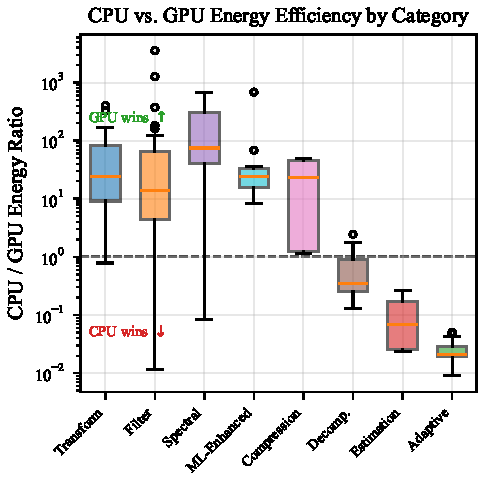
\includegraphics[width=\columnwidth]{figures/fig7_cpu_vs_gpu}
%\caption{CPU-to-GPU energy ratio across algorithm categories. GPU is more efficient for parallel algorithms (ratio $> 1$); CPU wins for sequential and decomposition algorithms.}
%\label{fig:cpugpu}
%\end{figure}

% =========================================================================
\section{Discussion}
\label{sec:discussion}
% =========================================================================

% TODO: Comparison to prior operation-counting literature
% Limitations (Kalman-vs-UKF flip, SVD/PCA cuSOLVER)
% Practical implications

% =========================================================================
\section{Conclusion}
\label{sec:conclusion}
% =========================================================================

% TODO: TOML extends to signal processing
% Kernel-launch counting for sequential overhead
% CPU vs GPU guidance

\bibliographystyle{IEEEbib}
\bibliography{refs}

\end{document}
